\clearpage
\subsection{Getting started with MOSL}
\texHeader
\hypertarget{static:starting tex}{}

\begin{itemize}

\item[$\blacktriangleright$] \hypertarget{static tex}{Begin a} new metamodel project from eclipse by navigating to the \texttt{New Metamodel} button on the
toolbar. In the dialog that appears, enter \texttt{LeitnersLearningBox} as the project name, and select \texttt{Textual (MOSL)}  (Fig.~\ref{fig:new_project}).

\begin{figure}[htbp]
	\centering
  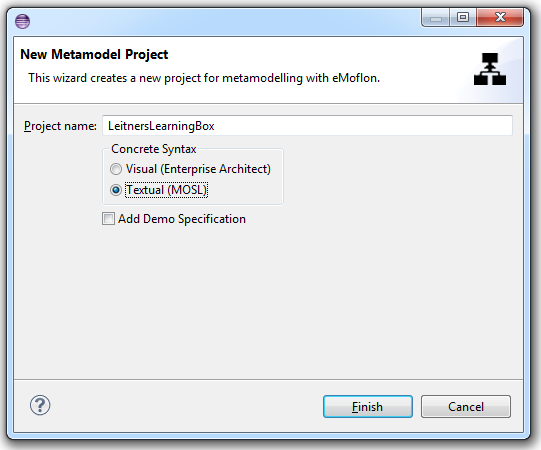
\includegraphics[width=0.7\textwidth]{eclipse_newMetamodelTextPlain}
	\caption{Create a new metamodeling project}
	\label{fig:new_project}
\end{figure}

\item[$\blacktriangleright$] Expand the project as deep as it goes. Your Package explorer may look different than ours (Fig.~\ref{fig:expanded_folders}),
depending on whether or not you completed the Demo in Part I. In an effort to keep things clear as possible, we have removed them from our workspaces, but
recommend keeping them for future reference.

\begin{figure}[htbp]
	\centering
  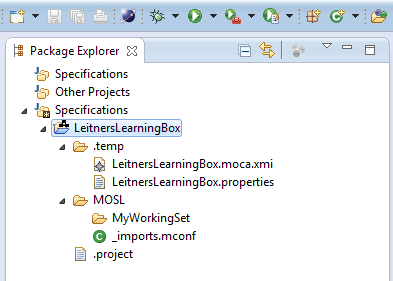
\includegraphics[width=0.5\textwidth]{eclipse_foldersExpanded}
	\caption{Expanded project files}
	\label{fig:expanded_folders}
\end{figure} 

\clearpage
\item[$\blacktriangleright$] You can see two folders, \texttt{.temp}, and \texttt{MOSL}, and one subfolder, \texttt{MyWorkingSet}, inside the
\texttt{Specifications} node\footnote{if you can't, make sure your \texttt{Top Level Elements} are set to \texttt{Working Sets}.}. We're most insterested in
\texttt{MyWorkingSet}, which stores the collection of files and  \emph{unifies} everything we need for Leitner's Box\footnote{for detailed review on the
explorer structure, review Part I.}.

\vspace{0.5cm}

\item[$\blacktriangleright$] Right click on your current workspace folder, \texttt{MyWorkingSet}, and create a new subfolder. Name it
`LearningBoxLanguage'. This is now the container for all your modelling files (Fig.~\ref{fig:all_files}).

\vspace{0.5cm}

\begin{figure}[htbp]
	\centering
  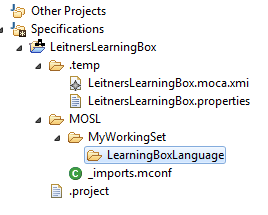
\includegraphics[width=0.4\textwidth]{eclipse_modelingContainer}
	\caption{Completed package explorer}
	\label{fig:all_files}
\end{figure} 

\vspace{0.5cm}

\item[$\blacktriangleright$] These are the basic steps needed to start any new textual metamodeling project. The \texttt{LearningBoxLanguage} folder will contain everything
your project needs such EClass files, pattern roots, and more. Remember, \texttt{MyWorkingSet} can hold several different projects at once, so files not within
\texttt{LearningBoxLanguage} will not be generated as part of that project.

\fancyfoot[R]{$\triangleright$ \hyperlink{static:classes tex}{Next}}

\end{itemize}
